\section{Reconstruction des points}
\begin{frame}{Reconstruction : retrouver les coordonnées 3D}
  \vspace*{\fill}
  \begin{itemize}
    \item<1-> On connaît les matrices de projection \( P_1 \) et \( P_2 \)
    \item<2-> Deux points image correspondants :
    \vspace*{-0.5em}
    \[
      m_1 = (u_1, v_1),\quad m_2 = (u_2, v_2)
    \]
    \item<3-> Point 3D inconnu :  \( M= (X , Y, Z) \)
    \item<4-> On a :
    \vspace*{-0.5em}
    \[
      \lambda_1 m_1 = P_1 M,\quad \lambda_2 m_2 = P_2 M
    \]
    \item<5-> Système de 6 équations linéaires homogènes
    \item<6-> Résolution par SVD
  \end{itemize}
  \vspace*{\fill}
\end{frame}



\begin{frame}{Reconstruction 3D multi-vues}
  \begin{minipage}{0.6\linewidth}
    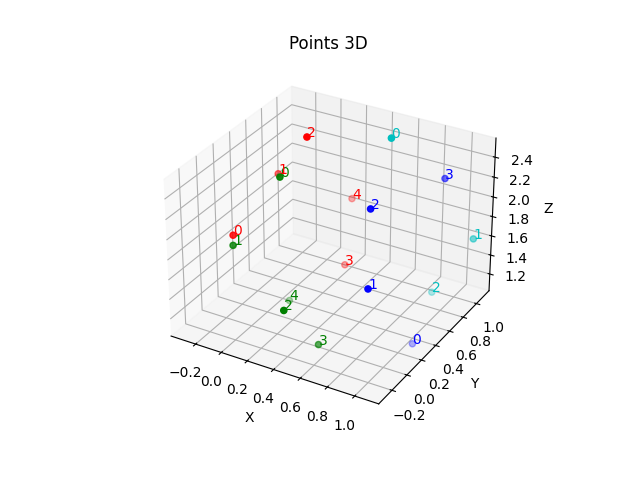
\includegraphics[width=\linewidth]{capture/cloud.png}
    \captionof*{figure}{Nuage de points}
  \end{minipage}
  \hfill
  \begin{minipage}{0.3\linewidth}
    \begin{minipage}{0.4\linewidth}
\fcolorbox{red}{white}{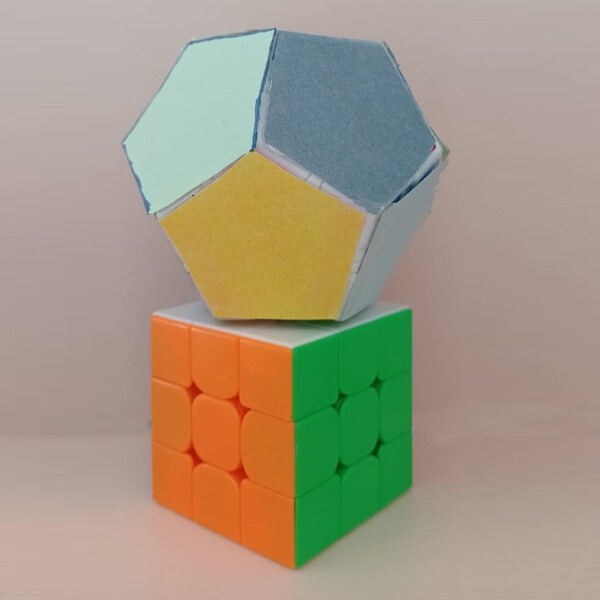
\includegraphics[width=\linewidth]{capture/dodecf1.jpg}}\\[0.5em]
      \fcolorbox{green!50!black}{white}{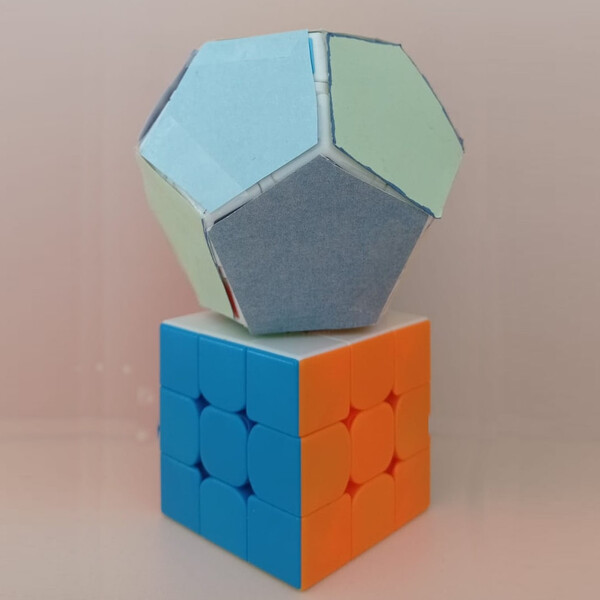
\includegraphics[width=\linewidth]{capture/dodecf3.jpg}}\\[0.5em]
      \fcolorbox{blue!50!black}{white}{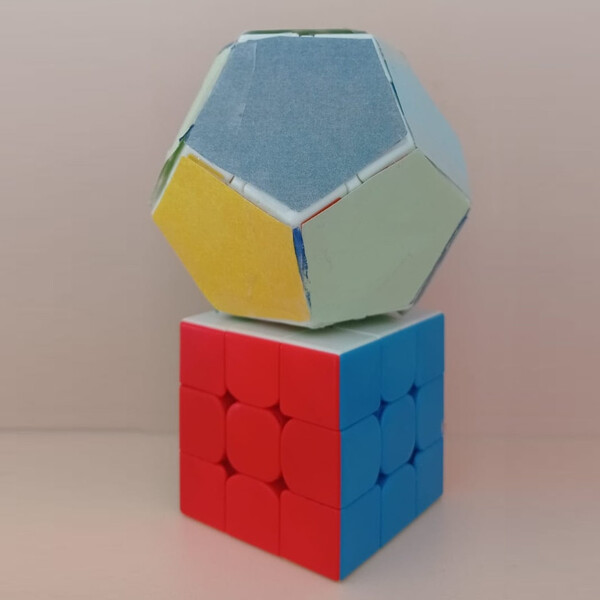
\includegraphics[width=\linewidth]{capture/dodecf5.jpg}}\\[0.5em]
      \fcolorbox{cyan}{white}{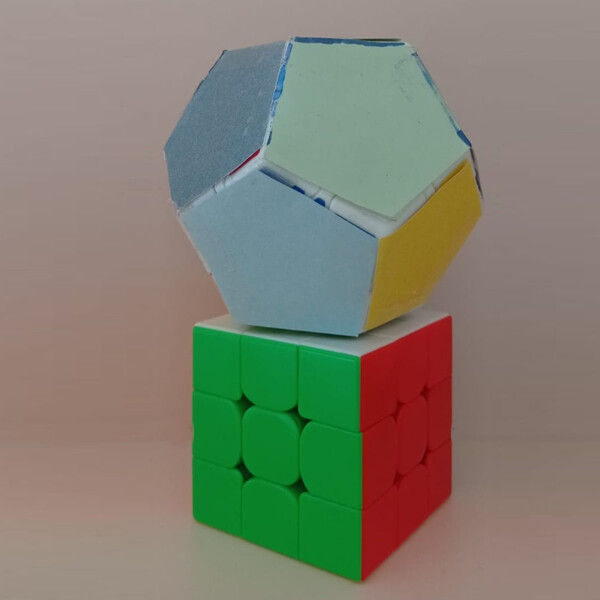
\includegraphics[width=\linewidth]{capture/dodecf7.jpg}}
    \end{minipage}
    \hfill
    \begin{minipage}{0.4\linewidth}
      \fcolorbox{red}{white}{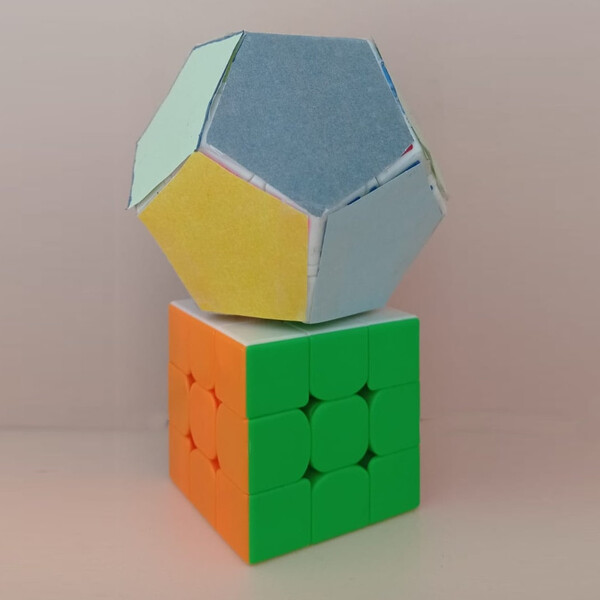
\includegraphics[width=\linewidth]{capture/dodecf0.jpg}}\\[0.5em]
      \fcolorbox{green!50!black}{white}{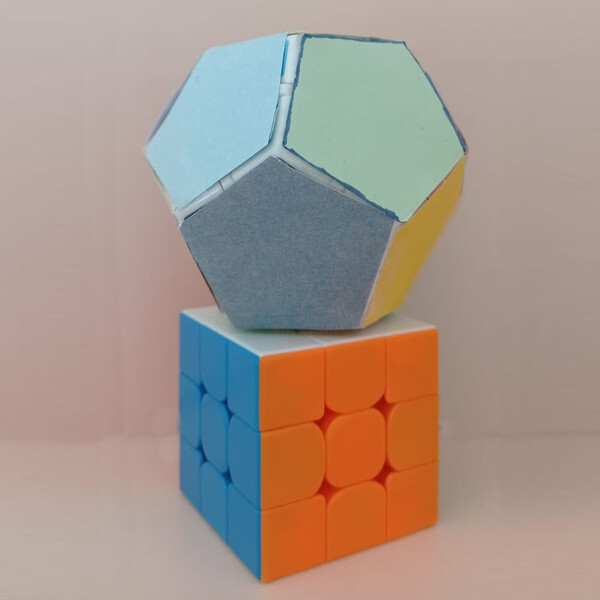
\includegraphics[width=\linewidth]{capture/dodecf2.jpg}}\\[0.5em]
      \fcolorbox{blue!50!black}{white}{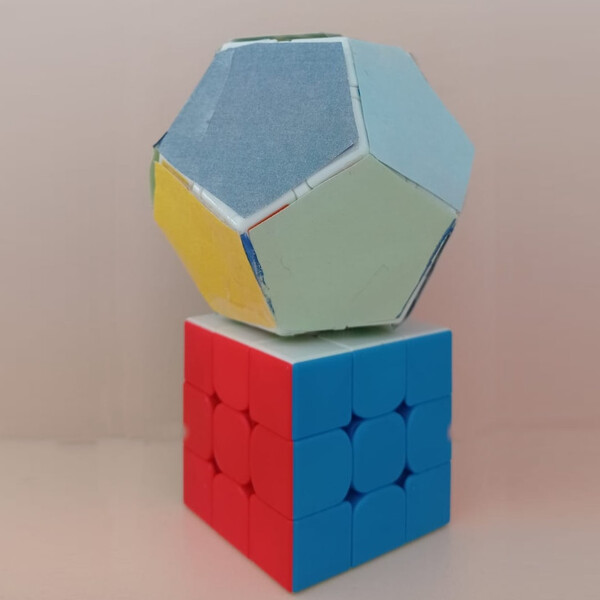
\includegraphics[width=\linewidth]{capture/dodecf4.jpg}}\\[0.5em]
      \fcolorbox{cyan}{white}{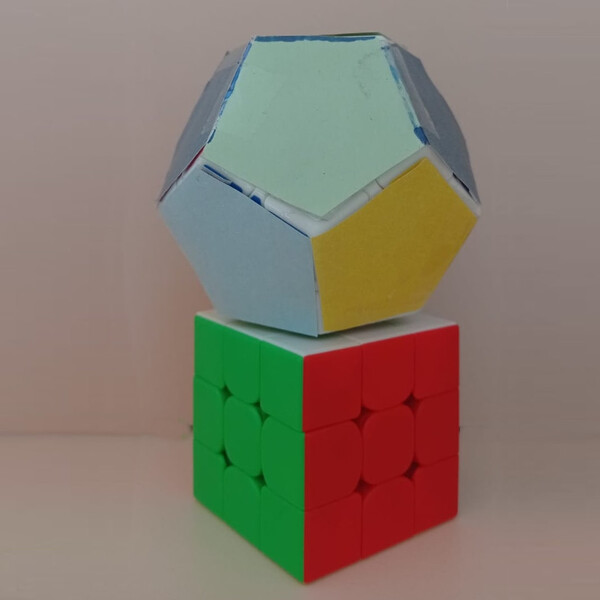
\includegraphics[width=\linewidth]{capture/dodecf6.jpg}}
    \end{minipage}
  \end{minipage}
\end{frame}